\documentclass[a4paper]{article}

\usepackage[english]{babel}
\usepackage{amsfonts, amssymb, mathtools, amsthm, amsmath}
\usepackage{graphicx, wrapfig, pgfplots}
\usepackage{url}
\usepackage[dvipsnames]{xcolor}
\usepackage{lastpage}

\usepackage[T1]{fontenc}
\usepackage{lmodern} % optional, safe default
\usepackage{newtxtext} % Times-like text + math

\usepackage{lastpage}

%loaded last
\usepackage[hidelinks]{hyperref}
\usepackage[nameinlink]{cleveref} 

\usepackage{siunitx}
  \sisetup{exponent-product = \cdot,
    output-decimal-marker = {,}}

%Giles Castelles incfig
\usepackage{import}
\usepackage{xifthen}
\usepackage{pdfpages}
\usepackage{transparent}

\newcommand{\incfig}[2][1]{%
  \def\svgwidth{#1\columnwidth}
  \import{./figures/}{#2.pdf_tex}
}

\setlength{\parindent}{0in}
\setlength{\parskip}{12pt}
\setlength{\oddsidemargin}{0in}
\setlength{\textwidth}{6.5in}
\setlength{\textheight}{8.8in}
\setlength{\topmargin}{0in}
\setlength{\headheight}{18pt}

\usepackage{fancyhdr}
\pagestyle{fancy}

\fancyhead{}
\fancyfoot{}
\fancyfoot[R]{\thepage{} of \pageref{LastPage}}
\fancyhead[L]{Alfred A, Benjamin, P \& Noah H}
\fancyhead[C]{Assignment w. 39--40}
\fancyhead[R]{October 22, 2025}

\pgfplotsset{compat=newest}

\pgfplotsset{every axis/.append style={
  axis x line=middle,    % put the x axis in the middle
  axis y line=middle,    % put the y axis in the middle
  axis line style={<->,color=black}, % arrows on the axis
}}

\usepackage{thmtools}
\usepackage{tcolorbox}
  \tcbuselibrary{skins, breakable}
  \tcbset{
    space to upper=1em,
    space to lower=1em,
  }

\theoremstyle{definition}

\newtcolorbox[auto counter]{definition}[1][]{%
  breakable,
  colframe=ForestGreen,  %frame color
  colback=ForestGreen!5, %background color
  colbacktitle=ForestGreen!25, %background color for title
  coltitle=ForestGreen!70!black,  %title color
  fonttitle=\bfseries\sffamily, %title font
  left=1em,              %space on left side in box,
  enhanced,              %more options
  frame hidden,          %hide frame
  borderline west={2pt}{0pt}{ForestGreen},  %display left line
  title=Definition \thetcbcounter: #1,
}

\newtcolorbox{greenline}{%
  breakable,
  colframe=ForestGreen,  %frame color
  colback=white,          %remove background color
  left=1em,              %space on left side in box
  enhanced,              %more options
  frame hidden,          %hide frame
  borderline west={2pt}{0pt}{ForestGreen},  %display left line
}

\newtcolorbox[auto counter, number within=section]{dis}[1][]{%
  breakable,
  colframe=NavyBlue,  %frame color
  colback=NavyBlue!5, %background color
  colbacktitle=NavyBlue!25,    %background color for title
  coltitle=NavyBlue!70!black,  %title color
  fonttitle=\bfseries\sffamily, %title font
  left=1em,            %space on left side in box,
  enhanced,            %more options
  frame hidden,        %hide frame
  borderline west={2pt}{0pt}{NavyBlue},  %display left line
  title=Discussion \thetcbcounter: #1
}

\newtcolorbox{blueline}{%
  breakable,
  colframe=NavyBlue,     %frame color
  colback=white,         %remove background
  left=1em,              %space on left side in box,
  enhanced,              %more options
  frame hidden,          %hide frame
  borderline west={2pt}{0pt}{NavyBlue},  %display left line
}

\newtcolorbox{exa}[1][]{%
  breakable,
  colframe=RawSienna,  %frame color
  colback=RawSienna!5, %background color
  colbacktitle=RawSienna!25,    %background color for title
  coltitle=RawSienna!70!black,  %title color
  fonttitle=\bfseries\sffamily, %title font
  left=1em,              %space on left side in box,
  enhanced,              %more options
  frame hidden,          %hide frame
  borderline west={2pt}{0pt}{RawSienna},  %display left line
  title=Example: #1,
}

\newtcolorbox[auto counter, number within=section]{sæt}[1][]{%
  breakable,
  colframe=RawSienna,  %frame color
  colback=RawSienna!5, %background color
  colbacktitle=RawSienna!25,    %background color for title
  coltitle=RawSienna!70!black,  %title color
  fonttitle=\bfseries\sffamily, %title font
  left=1em,              %space on left side in box,
  enhanced,              %more options
  frame hidden,          %hide frame
  borderline west={2pt}{0pt}{RawSienna},  %display left line
  title=Sætning \thetcbcounter: #1,
  before lower={\textbf{Bevis:}\par\vspace{0.5em}},
  colbacklower=RawSienna!25,
}

\newtcolorbox{redline}{%
  breakable,
  colframe=RawSienna,  %frame color
  colback=white,       %Remove background color
  left=1em,            %space on left side in box,
  enhanced,            %more options
  frame hidden,        %hide frame
  borderline west={2pt}{0pt}{RawSienna},  %display left line
}

\newtcolorbox{des}[1][]{%
  breakable,
  colframe=NavyBlue,  %frame color
  colback=NavyBlue!5, %background color
  colbacktitle=NavyBlue!25,    %background color for title
  coltitle=NavyBlue!70!black,  %title color
  fonttitle=\bfseries\sffamily, %title font
  left=1em,              %space on left side in box,
  enhanced,              %more options
  frame hidden,          %hide frame
  borderline west={2pt}{0pt}{NavyBlue},  %display left line
  title=Description of #1,
}

\makeatother
\def\@lecture{}%
\newcommand{\lecture}[3]{
  \ifthenelse{\isempty{#3}}{%
    \def\@lecture{Lecture #1}%
  }{%
    \def\@lecture{Lecture #1: #3}%
  }%
  \subsection*{\makebox[\textwidth][l]{\@lecture \hfill \normalfont\small\textsf{#2}}}
}

\makeatletter

\newcommand{\exercise}[1]{%
 \def\@exercise{#1}%
 \subsection*{Exercise #1}
}

\makeatother

%Format lim the same way in intext and in display
\let\svlim\lim\def\lim{\svlim\limits}

% horizontal rule
\newcommand\hr{
\noindent\rule[0.5ex]{\linewidth}{0.5pt}
}

\author{Alfred G. Andersen, Benjamin R. Pašalić \& Noah R. B. Hansen (Group Leader)}
\title{Take-Home Assignment weeks 39--40}
\date{October 22, 2025} 

\begin{document}

\begin{titlepage}
    \begin{center}
        \vspace*{1cm}
            
        \Huge{Take-Home Assignment week 37--38}
            
        \vspace{0.5cm}
        \LARGE{Statik \& Styrkelære}
        \vspace{1.5cm}
        \renewcommand{\arraystretch}{1.4}

        \normalsize{
          \begin{tabular}{c | c | c}
            Alfred Grue Andersen \quad & \quad Benjamin Rossavik Pašalić \quad & \quad Noah Rahbek Bigum Hansen \\
            202406227 & 202407403 & 202405538 \\
                      &Group Leader& 
          \end{tabular}
        }
        \vfill
            
        
\includegraphics[width=0.4\textwidth]{./figures/AU}
            
        \Large
        Mekanik \& Teknologi \\
        Aarhus Universitet \\
        Denmark \\
        October 22, 2025
            
    \end{center}
\end{titlepage}

\exercise{P10-1}
Determine the resultant internal loadings acting on the cross section at point $E$ of the handle arm, and on the cross section of the short link $BC$.
\begin{figure} [ht]
  \centering
  
\includegraphics[width=0.5\linewidth]{./figures/p10_1.png}
\end{figure}


\exercise{P10-2}
The bar has a cross-sectional area of \qty{400e-6}{\m\squared}. If it is subjected to a triangular axial distributed loading along its length which is $0$ at $x = 0$ and \qty{9}{\kN\per\m} at $x = \qty{1,5}{\m}$, and to two concentrated loads as shown, determine the average normal stress in the bas as a function of $x$ for $0 \leq 0 \leq \qty{0,6}{\m}$.

\begin{figure} [ht]
  \centering
  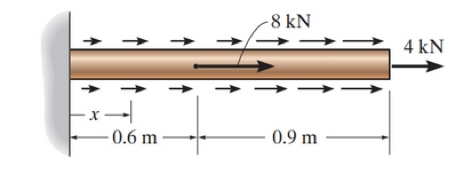
\includegraphics[width=0.5\linewidth]{./figures/p10_2.png}
\end{figure}


\exercise{P11-1}
Determine the required thickness of member $BC$ to the nearest \unit{\mm}, and the diameter of the pins at $A$ and $B$ if the allowable normal stress for member $BC$ is $\sigma_{\mathrm{allow}} = \qty{200}{\MPa}$ and the allowable shear stress for the pins is $\tau_{\text{allow}} = \qty{70}{\MPa}$.

\begin{figure} [ht]
  \centering
  
\includegraphics[width=0.5\linewidth]{./figures/p11_1.png}
\end{figure}


\exercise{P11-2}
Nylon strips are fused to glass plates. When moderately heated the nylon will become soft while the glass stays approximately rigid. Determine the average shear strain in the nylon due to the load $P$ when the assembly deforms as indicated.

\begin{figure} [ht]
  \centering
  
\includegraphics[width=0.5\linewidth]{./figures/p11_2.png}
\end{figure}

\exercise{P12-1}
The rigid beam is supported by the three suspender bars. Bars $AB$ and $EF$ are made of aluminum and bar $CD$ is made of steel. If each bar has a cross-sectional area of \qty{450}{\mm\squared}, determine the maximum value of $P$ if the allowable stress is $\left( \sigma_{\text{allow}} \right)_{\text{st}} = \qty{200}{\MPa} $ for the steel and $\left( \sigma_{\text{allow}} \right)_{\text{al}} = \qty{150}{\MPa} $ for the aluminum. $E_{\text{st}} = \qty{200}{\GPa}$ and $E_{\text{al}} = \qty{70}{\GPa}$.

\begin{figure} [ht]
  \centering
  
\includegraphics[width=0.5\linewidth]{./figures/p12_1.png}
\end{figure}

\end{document}
